% Created by tikzDevice version 0.12 on 2019-01-30 14:23:54
% !TEX encoding = UTF-8 Unicode
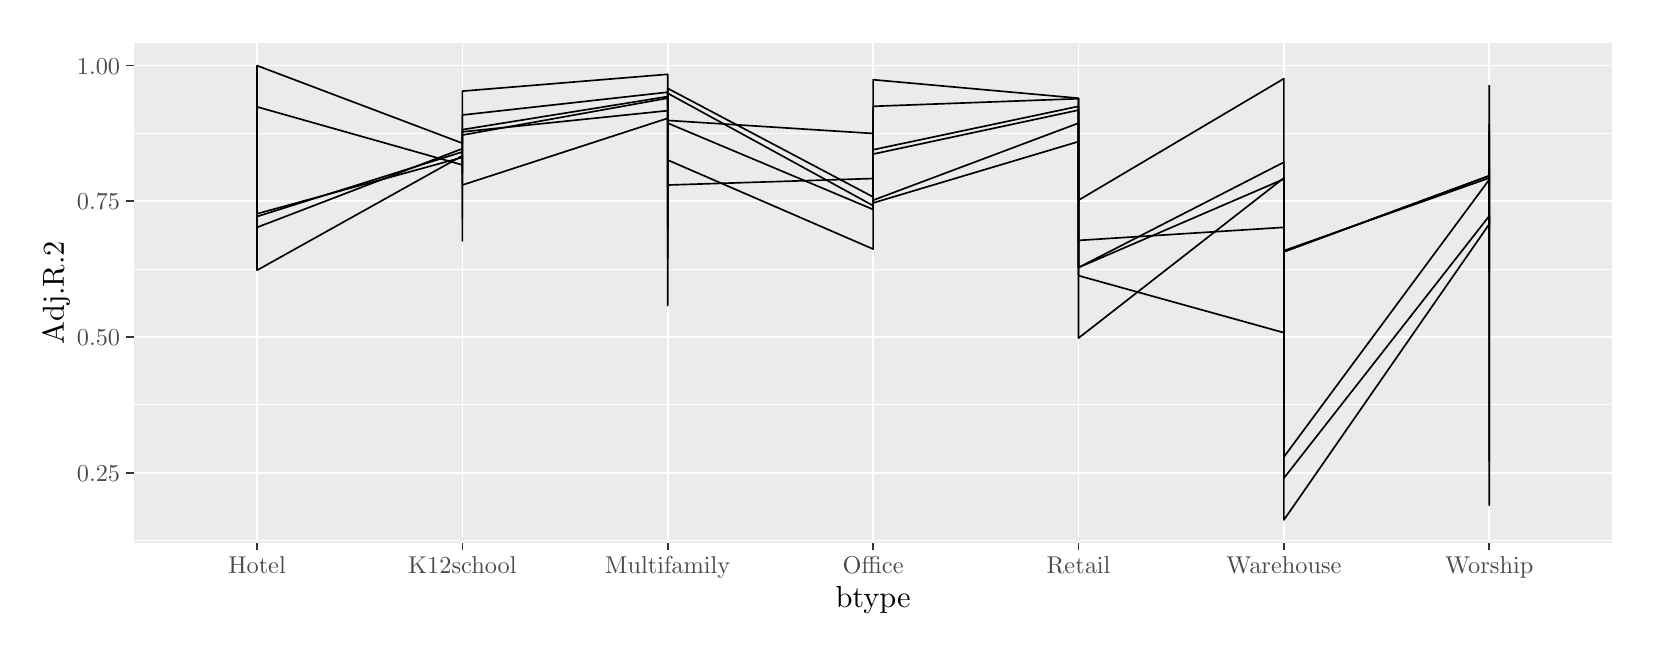
\begin{tikzpicture}[x=1pt,y=1pt]
\definecolor{fillColor}{RGB}{255,255,255}
\path[use as bounding box,fill=fillColor,fill opacity=0.00] (0,0) rectangle (578.16,216.81);
\begin{scope}
\path[clip] (  0.00,  0.00) rectangle (578.16,216.81);
\definecolor{drawColor}{RGB}{255,255,255}
\definecolor{fillColor}{RGB}{255,255,255}

\path[draw=drawColor,line width= 0.6pt,line join=round,line cap=round,fill=fillColor] (  0.00,  0.00) rectangle (578.16,216.81);
\end{scope}
\begin{scope}
\path[clip] ( 38.36, 30.72) rectangle (572.66,211.31);
\definecolor{fillColor}{gray}{0.92}

\path[fill=fillColor] ( 38.36, 30.72) rectangle (572.66,211.31);
\definecolor{drawColor}{RGB}{255,255,255}

\path[draw=drawColor,line width= 0.3pt,line join=round] ( 38.36, 31.48) --
	(572.66, 31.48);

\path[draw=drawColor,line width= 0.3pt,line join=round] ( 38.36, 80.51) --
	(572.66, 80.51);

\path[draw=drawColor,line width= 0.3pt,line join=round] ( 38.36,129.55) --
	(572.66,129.55);

\path[draw=drawColor,line width= 0.3pt,line join=round] ( 38.36,178.58) --
	(572.66,178.58);

\path[draw=drawColor,line width= 0.6pt,line join=round] ( 38.36, 56.00) --
	(572.66, 56.00);

\path[draw=drawColor,line width= 0.6pt,line join=round] ( 38.36,105.03) --
	(572.66,105.03);

\path[draw=drawColor,line width= 0.6pt,line join=round] ( 38.36,154.07) --
	(572.66,154.07);

\path[draw=drawColor,line width= 0.6pt,line join=round] ( 38.36,203.10) --
	(572.66,203.10);

\path[draw=drawColor,line width= 0.6pt,line join=round] ( 82.89, 30.72) --
	( 82.89,211.31);

\path[draw=drawColor,line width= 0.6pt,line join=round] (157.09, 30.72) --
	(157.09,211.31);

\path[draw=drawColor,line width= 0.6pt,line join=round] (231.30, 30.72) --
	(231.30,211.31);

\path[draw=drawColor,line width= 0.6pt,line join=round] (305.51, 30.72) --
	(305.51,211.31);

\path[draw=drawColor,line width= 0.6pt,line join=round] (379.72, 30.72) --
	(379.72,211.31);

\path[draw=drawColor,line width= 0.6pt,line join=round] (453.93, 30.72) --
	(453.93,211.31);

\path[draw=drawColor,line width= 0.6pt,line join=round] (528.14, 30.72) --
	(528.14,211.31);
\definecolor{drawColor}{RGB}{0,0,0}

\path[draw=drawColor,line width= 0.6pt,line join=round] ( 82.89,181.13) --
	( 82.89,152.89) --
	( 82.89,188.20) --
	(157.09,167.21) --
	(157.09,139.75) --
	(157.09,179.17) --
	(231.30,186.82) --
	(231.30,116.41) --
	(231.30,168.97) --
	(305.51,136.81) --
	(305.51,176.82) --
	(305.51,153.48) --
	(379.72,175.64) --
	(379.72,162.30) --
	(379.72,127.20) --
	(453.93,106.60) --
	(453.93, 82.87) --
	(453.93, 38.93) --
	(528.14,145.83) --
	(528.14,166.42);

\path[draw=drawColor,line width= 0.6pt,line join=round] ( 82.89,190.35) --
	( 82.89,149.56) --
	(157.09,169.95) --
	(157.09,160.15) --
	(157.09,178.00) --
	(231.30,191.33) --
	(231.30,159.17) --
	(231.30,182.31) --
	(305.51,151.12) --
	(305.51,180.15) --
	(305.51,172.70) --
	(379.72,188.39) --
	(379.72,168.97) --
	(379.72,139.94) --
	(453.93,144.65) --
	(453.93, 84.44) --
	(453.93,136.22) --
	(528.14,162.50) --
	(528.14, 44.23) --
	(528.14,181.92);

\path[draw=drawColor,line width= 0.6pt,line join=round] ( 82.89,189.57) --
	( 82.89,148.57) --
	(157.09,171.92) --
	(157.09,164.07) --
	(157.09,179.96) --
	(231.30,191.92) --
	(231.30,182.90) --
	(231.30,193.10) --
	(305.51,152.50) --
	(305.51,182.11) --
	(305.51,188.39) --
	(379.72,191.14) --
	(379.72,171.52) --
	(379.72,130.14) --
	(453.93,162.11) --
	(453.93, 88.75) --
	(453.93,135.83) --
	(528.14,163.29) --
	(528.14,128.57);

\path[draw=drawColor,line width= 0.6pt,line join=round] ( 82.89,190.74) --
	( 82.89,144.65) --
	(157.09,173.09) --
	(157.09,164.46) --
	(157.09,185.25) --
	(231.30,193.49) --
	(231.30,188.59) --
	(231.30,194.86) --
	(305.51,155.64) --
	(305.51,183.10) --
	(305.51,198.00) --
	(379.72,191.33) --
	(379.72,172.31) --
	(379.72,130.14) --
	(453.93,168.19) --
	(453.93, 87.77) --
	(453.93,135.83) --
	(528.14,163.29) --
	(528.14,196.04);

\path[draw=drawColor,line width= 0.6pt,line join=round] ( 82.89,175.45) --
	( 82.89,155.44) --
	( 82.89,129.16) --
	(157.09,170.54) --
	(157.09,147.79) --
	(157.09,159.95) --
	(231.30,184.08) --
	(231.30,144.65) --
	(231.30,159.95) --
	(305.51,162.30) --
	(305.51,182.90) --
	(305.51,154.46) --
	(379.72,182.31) --
	(379.72,131.31) --
	(379.72,104.64) --
	(453.93,162.50) --
	(453.93, 74.04) --
	(453.93, 54.04) --
	(528.14,148.77) --
	(528.14, 60.31) --
	(528.14,101.70);

\path[draw=drawColor,line width= 0.6pt,line join=round] ( 82.89,191.33) --
	( 82.89,172.31) --
	( 82.89,203.10) --
	(157.09,175.05) --
	(157.09,181.53) --
	(157.09,193.88) --
	(231.30,199.96) --
	(231.30,133.47) --
	(231.30,183.29) --
	(305.51,178.58) --
	(305.51,186.82) --
	(305.51,171.13) --
	(379.72,187.02) --
	(379.72,156.22) --
	(379.72,154.46) --
	(453.93,198.39) --
	(453.93,113.27) --
	(453.93, 61.69) --
	(528.14,161.91) --
	(528.14,144.46) --
	(528.14,179.37);
\end{scope}
\begin{scope}
\path[clip] (  0.00,  0.00) rectangle (578.16,216.81);
\definecolor{drawColor}{gray}{0.30}

\node[text=drawColor,anchor=base east,inner sep=0pt, outer sep=0pt, scale=  0.88] at ( 33.41, 52.97) {0.25};

\node[text=drawColor,anchor=base east,inner sep=0pt, outer sep=0pt, scale=  0.88] at ( 33.41,102.00) {0.50};

\node[text=drawColor,anchor=base east,inner sep=0pt, outer sep=0pt, scale=  0.88] at ( 33.41,151.04) {0.75};

\node[text=drawColor,anchor=base east,inner sep=0pt, outer sep=0pt, scale=  0.88] at ( 33.41,200.07) {1.00};
\end{scope}
\begin{scope}
\path[clip] (  0.00,  0.00) rectangle (578.16,216.81);
\definecolor{drawColor}{gray}{0.20}

\path[draw=drawColor,line width= 0.6pt,line join=round] ( 35.61, 56.00) --
	( 38.36, 56.00);

\path[draw=drawColor,line width= 0.6pt,line join=round] ( 35.61,105.03) --
	( 38.36,105.03);

\path[draw=drawColor,line width= 0.6pt,line join=round] ( 35.61,154.07) --
	( 38.36,154.07);

\path[draw=drawColor,line width= 0.6pt,line join=round] ( 35.61,203.10) --
	( 38.36,203.10);
\end{scope}
\begin{scope}
\path[clip] (  0.00,  0.00) rectangle (578.16,216.81);
\definecolor{drawColor}{gray}{0.20}

\path[draw=drawColor,line width= 0.6pt,line join=round] ( 82.89, 27.97) --
	( 82.89, 30.72);

\path[draw=drawColor,line width= 0.6pt,line join=round] (157.09, 27.97) --
	(157.09, 30.72);

\path[draw=drawColor,line width= 0.6pt,line join=round] (231.30, 27.97) --
	(231.30, 30.72);

\path[draw=drawColor,line width= 0.6pt,line join=round] (305.51, 27.97) --
	(305.51, 30.72);

\path[draw=drawColor,line width= 0.6pt,line join=round] (379.72, 27.97) --
	(379.72, 30.72);

\path[draw=drawColor,line width= 0.6pt,line join=round] (453.93, 27.97) --
	(453.93, 30.72);

\path[draw=drawColor,line width= 0.6pt,line join=round] (528.14, 27.97) --
	(528.14, 30.72);
\end{scope}
\begin{scope}
\path[clip] (  0.00,  0.00) rectangle (578.16,216.81);
\definecolor{drawColor}{gray}{0.30}

\node[text=drawColor,anchor=base,inner sep=0pt, outer sep=0pt, scale=  0.88] at ( 82.89, 19.71) {Hotel};

\node[text=drawColor,anchor=base,inner sep=0pt, outer sep=0pt, scale=  0.88] at (157.09, 19.71) {K12school};

\node[text=drawColor,anchor=base,inner sep=0pt, outer sep=0pt, scale=  0.88] at (231.30, 19.71) {Multifamily};

\node[text=drawColor,anchor=base,inner sep=0pt, outer sep=0pt, scale=  0.88] at (305.51, 19.71) {Office};

\node[text=drawColor,anchor=base,inner sep=0pt, outer sep=0pt, scale=  0.88] at (379.72, 19.71) {Retail};

\node[text=drawColor,anchor=base,inner sep=0pt, outer sep=0pt, scale=  0.88] at (453.93, 19.71) {Warehouse};

\node[text=drawColor,anchor=base,inner sep=0pt, outer sep=0pt, scale=  0.88] at (528.14, 19.71) {Worship};
\end{scope}
\begin{scope}
\path[clip] (  0.00,  0.00) rectangle (578.16,216.81);
\definecolor{drawColor}{RGB}{0,0,0}

\node[text=drawColor,anchor=base,inner sep=0pt, outer sep=0pt, scale=  1.10] at (305.51,  7.44) {btype};
\end{scope}
\begin{scope}
\path[clip] (  0.00,  0.00) rectangle (578.16,216.81);
\definecolor{drawColor}{RGB}{0,0,0}

\node[text=drawColor,rotate= 90.00,anchor=base,inner sep=0pt, outer sep=0pt, scale=  1.10] at ( 13.08,121.02) {Adj.R.2};
\end{scope}
\end{tikzpicture}
